\chapter{Méthodologie de travail}
\markboth{Chapitre 3. Méthodologie de travail}{} 
\begin{spacing}{1.2}
\minitoc
\thispagestyle{MyStyle}
\end{spacing}
\newpage

\section*{Introduction}
Créer une plateforme est un défi complexe qui nécessite une approche méthodique et efficace. Dans cette optique, nous avons adopté une méthodologie de gestion de projet dénommé Scrum. Cette méthodologie favorise la flexibilité, la collaboration et la livraison continue de fonctionnalités. Au cœur de notre approche réside une méthode itérative et incrémentale qui nous permet de répondre aux besoins évolutifs de notre projet tout en garantissant un développement rapide et efficace.\par

Dans ce chapitre, nous plongerons au cœur de notre méthodologie de travail, détaillant les principes directeurs, les processus et les pratiques adopté pour mener à bien la création de notre plateforme de bibliothèque numérique. En présentant notre méthodologie de manière détaillée, nous visons à offrir un aperçu complet de notre processus de développement, mettant en lumière les stratégies que nous avons adoptées pour assurer le succès de notre projet.
\par
\section{Présentation de la méthodologie agile Scrum}
La méthodologie Agile Scrum est une approche de gestion de projet qui vise à favoriser la flexibilité, la réactivité et la collaboration dans le développement de produits logiciels et de solutions complexes. Contrairement aux méthodologies traditionnelles, Scrum privilégie une approche itérative et incrémentale, où le travail est organisé en cycles courts appelés "sprints"[biblio].
	Au cœur de cette méthodologie se trouvent trois principaux acteurs dont nous endosserons le rôle : le Product Owner, l'Équipe de développement et le Scrum Master. Le Product Owner est chargé de définir les objectifs du projet et de prioriser les fonctionnalités à développer, en se basant sur les besoins du client et les retours utilisateurs. L'Équipe de développement est responsable de la réalisation des tâches et de la livraison des fonctionnalités lors de chaque sprint. Le Scrum Master, quant à lui, est garant du respect des principes Scrum, il facilite les interactions au sein de l'équipe et veille à ce que les processus Scrum soient bien compris et suivis.
La méthodologie Scrum repose également sur un ensemble d'artefacts et d'événements clés. Les principaux artefacts incluent le Product Backlog, qui recense toutes les fonctionnalités à développer, et le Sprint Backlog, qui contient les tâches à réaliser lors de chaque sprint. Les événements Scrum comprennent la Planification du Sprint, qui définit les objectifs du sprint, le Daily Scrum, une réunion quotidienne pour synchroniser le travail de l'équipe, la Revue de Sprint, où les fonctionnalités développées sont présentées au Product Owner, et la Rétrospective de Sprint, qui permet à l'équipe de réfléchir et de s'améliorer continuellement.
En résumé, la méthodologie Agile Scrum offre une approche structurée et adaptable pour gérer efficacement les projets complexes. En favorisant la maneabilité, et la livraison continue de valeur, Scrum permet au développeur d'organiser et de générer plus facilement les tâches à travers des solutions adaptatives pour des problèmes complexes \cite{schwaber2011scrum}.
	
	\begin{figure}[H]%
    \center%
    \setlength{\fboxsep}{5pt}%
    \setlength{\fboxrule}{0.5pt}%
    \fbox{
    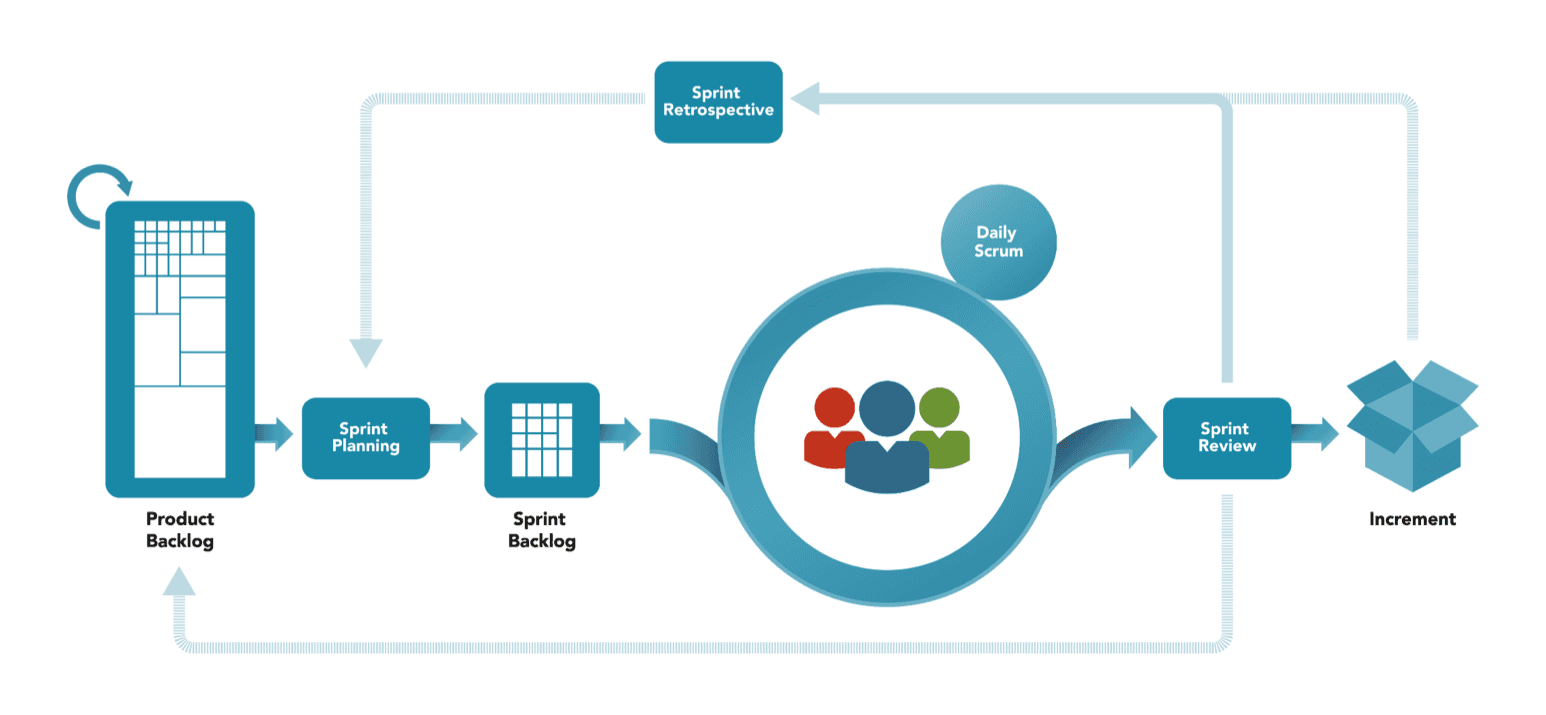
\includegraphics[width=12.5cm,height=9cm]{images/scrum.png}%
    }
    \caption{Fonctionnement de la méthodologie agile scrum}%
\end{figure} \par

\section*{Conclusion}

En adoptant la méthodologie Scrum, notre objectif a été de créer un environnement de travail agile où l'adaptabilité, la transparence et la communication étaient au cœur de notre processus de développement. En nous appuyant sur les valeurs de Scrum telles que le respect, l'engagement et le courage, nous avons relevé avec succès les défis complexes de notre projet tout en restant alignés sur nos objectifs.
À mesure que nous avons avancé dans notre projet, la méthodologie Agile Scrum nous a permis de livrer rapidement des fonctionnalités utilisables et de répondre de manière proactive aux besoins changeants de notre marché. En embrassant les principes de Scrum, nous sommes resté confiants dans notre capacité à créer une plateforme de bibliothèque numérique innovante, robuste et adaptée aux besoins de notre communauté d'utilisateurs.
\par